\documentclass[11pt]{article}
\usepackage[margin=25mm]{geometry}
\usepackage{fontspec,unicode-math,mathtools,siunitx,booktabs,csquotes,listings,tikz,microtype}
\setmainfont{lmroman10-regular.otf}[BoldFont=lmroman10-bold.otf,ItalicFont=lmroman10-italic.otf,BoldItalicFont=lmroman10-bolditalic.otf]
\setsansfont{lmsans10-regular.otf}[BoldFont=lmsans10-bold.otf,ItalicFont=lmsans10-oblique.otf,BoldItalicFont=lmsans10-boldoblique.otf]
\setmonofont{lmmono10-regular.otf}[ItalicFont=lmmono10-italic.otf]
\setmathfont{latinmodern-math.otf}
\usepackage{hyperref}
\usepackage[nameinlink]{cleveref}
\usepackage[backend=biber,style=numeric,sorting=none]{biblatex}
\addbibresource{references.bib}
\title{Neruda compatibility fixture: theoretical illustration}
\author{Synthetic fixture; no research authorship asserted}
\date{Compatibility experiment}
\begin{document}
\maketitle
\begin{abstract}
This synthetic document exercises typesetting dependencies. Its numerical
values are exact illustrations, not experimental measurements.
\end{abstract}
\section{Mathematical concepts}
For a dimensionless affine mapping,
\begin{equation}\label{eq:affine}
 y(x)=a x+b.
\end{equation}
\begin{description}
\item[$y$] Output function from the real numbers to the real numbers.
\item[$x$] Dimensionless real input.
\item[$a$] Dimensionless slope, fixed at two.
\item[$b$] Dimensionless intercept, fixed at one.
\end{description}
The mapping doubles the input and adds one. At zero it returns one;
at one it returns three. These are deterministic checks, not estimates.
\section{Illustrative values}
\begin{table}[ht]
\centering
\begin{tabular}{rr}\toprule Input & Output\\\midrule
0 & 1\\1 & 3\\2 & 5\\\bottomrule\end{tabular}
\caption{Exact synthetic values of \cref{eq:affine}.}\label{tab:values}
\end{table}
\begin{center}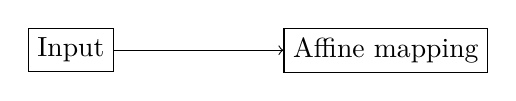
\begin{tikzpicture}
\node[draw] (input) at (0,0) {Input};
\node[draw] (output) at (4,0) {Affine mapping};
\draw[->] (input) -- (output);
\end{tikzpicture}\end{center}
Unicode text: café; semantic quantity: \SI{10}{\micro\metre}.
Vector and matrix typography: $\symbf{x}$, $\symbf{A}$.
\section{Reproducibility and limitations}
\Cref{tab:values} is hand-computable. No sampling uncertainty, treatment
effect, or biological result is claimed. The cited documentation describes
Tectonic's command interface \cite{tectonic-interface}; it is not evidence
for a scientific finding. Toolchain observations belong in the build receipt.
\printbibliography
\end{document}
